%!TEX root = ../main.tex

\chapter{Literature Review}\label{cha:literature}

% Brief 1 para intro
\section{Deep Learning}\label{sec:deep_learning_lit}
% section on history of deep learning up to recent cutting edge developments

\subsection{Training Deep Neural Networks}\ref{subsec:training}
Due to the size of deep neural networks, and the non-convexity of the parameters, finding good optima has always been a challenge.
Stochastic gradient descent (SGD) has remained a popular strategy for researchers since the 80's although many optimisation algorithms are now used.
These include Adam \cite{Kingma_Ba_2014}, ADADELTA \cite{Zeiler_2012} and AdaGrad \cite{Duchi_Hazan_Singer_2011}.
For all of the optimisers mentioned, one of the main issues during training is choosing an appropriate learning rate.

It has been suggested by Dauphin et al. in \cite{Dauphin_de_Vries_Bengio_2015} that saddle points cause issues during training, not poor local optima.
However, in The Deep Learning Book \cite{Goodfellow-et-al-2016}, Goodfellow et al. prove that although learning is slow around saddle points due to the flattness, gradient based optimisation algorithms are still able to escape.

could use linear cyclical: \cite{Smith_2015}

cosine annealing/restarts \cite{Loshchilov_Hutter_2016}

Snapshots Ensemble: Train 1, get M for free \cite{Huang_Li_Pleiss_Liu_Hopcroft_Weinberger_2017}

In \cite{Keskar_Mudigere_Nocedal_Smelyanskiy_Tang_2016} it is suggested that convergence to sharp minima leads to poor generalisation for deep learning.
Figure \ref{fig:wide_optima} outlines a sharp minimum.
Numerical evidence is then given that supports this view and several attempts to address the problem are presented.
However, initial results suggest that whilst these strategies do lead to better generalisation, they still converge to sharp minima.

\begin{figure}
    \centering
    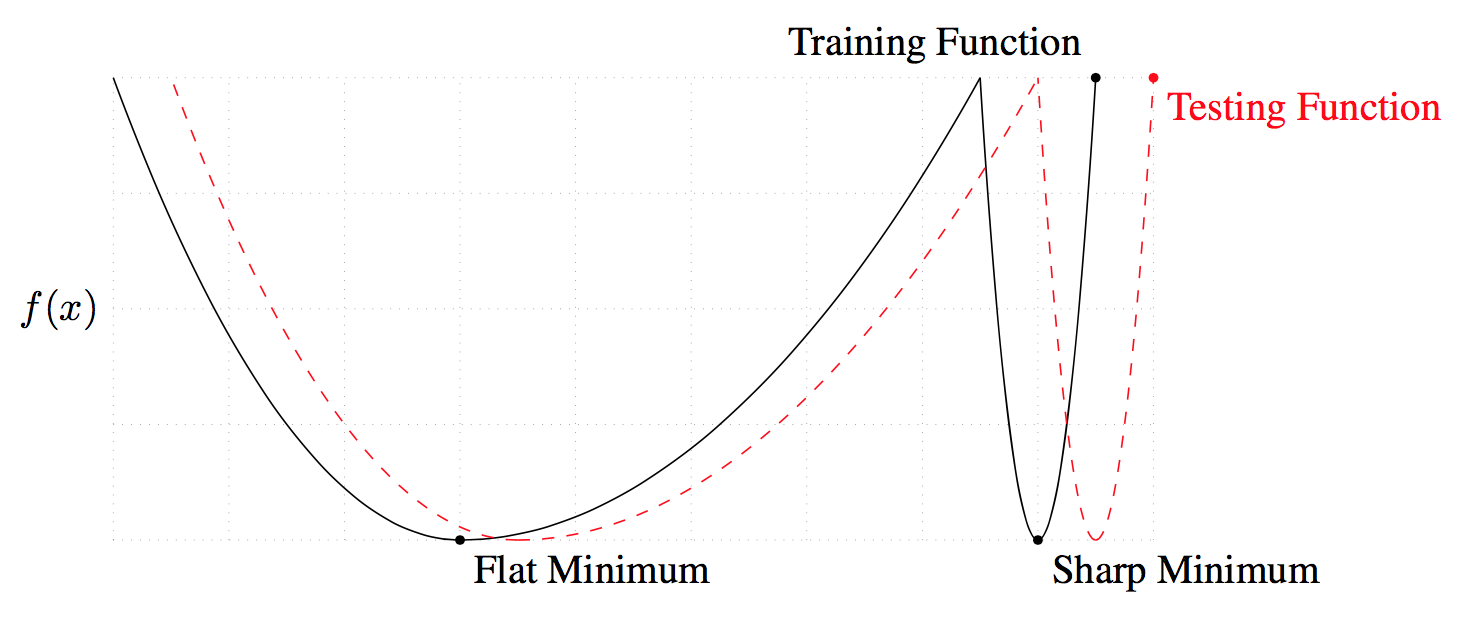
\includegraphics[width=\textwidth]{./img/Wide_optima.png}
    \caption{A Conceptual Sketch of Flat and Sharp Minima. The Y-axis indicates value of the loss function and the X-axis the variables (parameters) \cite{Keskar_Mudigere_Nocedal_Smelyanskiy_Tang_2016}}
    \label{fig:wide_optima}
\end{figure}


\subsection{Recent Developments}\label{subsec:recent_improvements}
In late 2017, Hinton outlined a method for training capsule based methods.
This is something he'd been thinking about for years.
It learns pose representations of objects.

People are well aware that ensemble methods produce great results.
Blah Blah outlined a method where models where saved periodically (Snapshot).
The period was large enough such that the models performed better/worse in different areas.
At prediction time they could be used as an ensemble.

(FGE) Someone else then showed that making the cycles short was still pretty good.
This is because because there exist connected paths of low loss between sufficiently different models, it is possible to travel along those paths in small steps and the models encountered along will be different enough to allow ensembling them with good results.
This is much faster



\begin{figure}
    \centering
    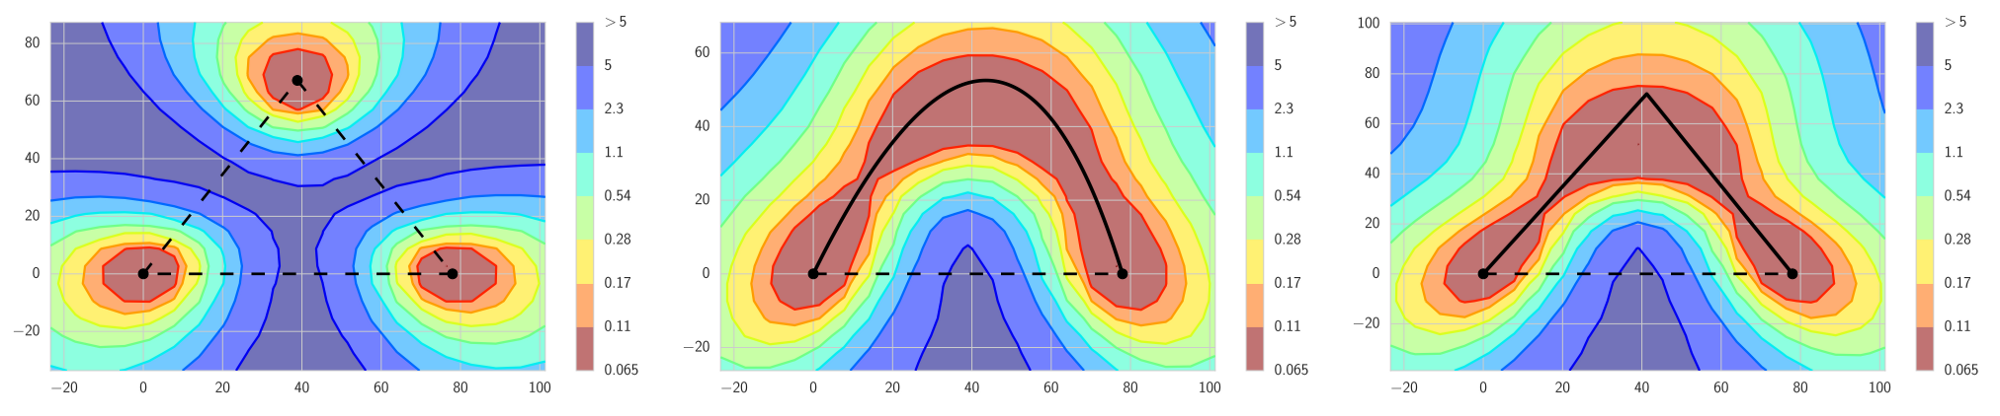
\includegraphics[width=\textwidth]{./img/FGE.png}
    \caption{\cite{Garipov_Izmailov_Podoprikhin_Vetrov_Wilson_2018}}
    \label{fig:FGE_shortest_path}
\end{figure}

\begin{figure}
    \centering
    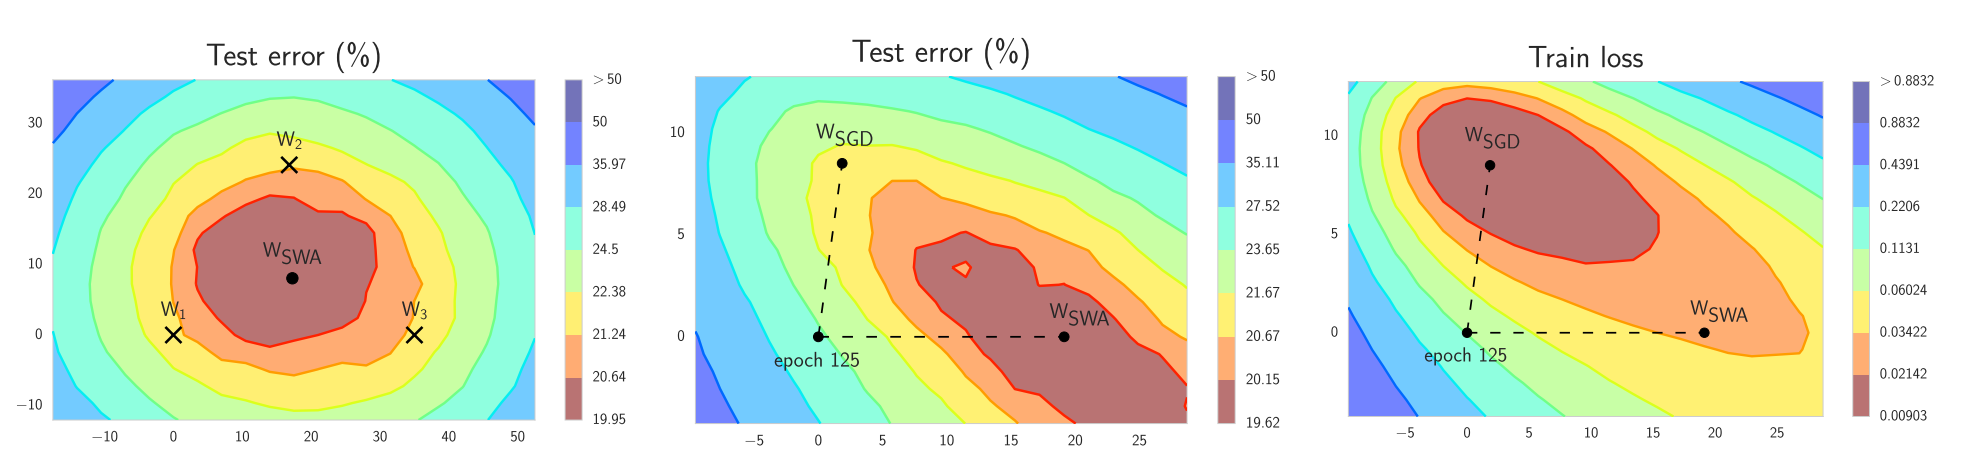
\includegraphics[width=\textwidth]{./img/SWA.png}
    \caption{\cite{Izmailov_Podoprikhin_Garipov_Vetrov_Wilson_2018}}
    \label{fig:SWA}
\end{figure}

This is all taking an ensemble in model space, what if we do it in weight space.
We find that maintaining an average of the weights we encouter performs pretty well; it is better than snapshot and almost as good as FGE
This is much quicker and less computationally expensive because we don't have to carry around several different models.

\section{Deep Learning in Medicine}\label{deep_learning_medic_lit}
% section on deep learning in medicine
U-Net \cite{Ronneberger_Fischer_Brox_2015}